\chapter{Model Evaluation on KIS Task}\label{chap:evaluation}
In Chapter \ref{chap:retrieval_model} we evaluated our model on classification task which differs from KIS task. In this chapter, we, therefore, discuss the differences between classification and known-item search, propose possible evaluation methods and present their results. We also show and discuss this year's Video Browser Showdown competition we successfully participated in.

In KIS task the goal of a retrieval model parametrized by $\bm{\kappa}$ is to minimize a position (or rank) $r$ of the searched image $\bm{x}$ given a user query $Q$. If the position is treated as a random variable the objective can be written as
\begin{equation}
\mathop{\arg\max}_{\bm{\kappa}}\mathbb{E}_{\left(\bm{x},Q\right)\sim \hat{p}_{data}}\left[
\sum_{t=1}^{|C|}p_{model}\left(r\leq t\given\bm{x}, Q;\bm{\kappa}\right)
\right]\label{eq:kis}
\end{equation}
where $p_{model}\left(r\leq t\given\cdot\right)$ is a probability image's position is less than or equal to~$t$ and $|C|$ is size of the collection. Intuitively, the ideal user constructing the most specific queries~$Q$ for images~$\bm{x}$ together paired with an ideal model capable of distinguishing all images from each other would always have ${p_{model}\left(r\leq 1\right)=1}$, therefore yielding the highest possible value. Unfortunately, unlike the function~\ref{eq:mle} of the classification task, function~\ref{eq:kis} is not differentiable thus we can only use it as a quality measure of our model. Yet another issue arises with $\hat{p}_{data}$ distribution since it is dependent on a set of supported labels and on a dataset, the images $\bm{x}$ are taken from. In order to evaluate our model, a thorough user study would be needed yet a slight change to the model could nullify its results. In the next section, we construct simple simulations providing us with an insight into model's performance without the need for a broad study.

\section{User Simulations}
To simplify the simulations only queries containing \textsf{OR} will be considered. We can, therefore, write $Q=\{N_1\}$ and for a sake of simplicity, we will use $Q=N_1\subseteq L_m$.
We take inspiration from~\cite{kovalvcik2017comparison} on approaches toward generating user queries and define the following users:
\begin{description}[labelwidth=1em, leftmargin=!]
	\item \textbf{Network User.} Assumes a user is coherent with the model $\bm{\theta}$. Query $Q_{n}$ of length~$|Q_{n}|$ for a random image $\bm{x}$ is generated by drawing $|Q_{n}|$-times from set $\{1,\dots,L_m\}$ with probability $p(label)=\bm{\hat{y}}_{label}$ where $\bm{\hat{y}}=f\left(\bm{x}; \bm{\theta}\right)$ is the distribution of classes predicted by our neural network.
	\item \textbf{Real User.} A human judge is given a random image $\bm{x}$ from a dataset and describes it in a set of labels $Q_r\subseteq L_m$ generating one $(\bm{x},Q_r)$ pair.
	\item \textbf{Distribution User.} Given a set of image-query pairs generated by humans we can infer distribution $\mathcal{C}$ how likely user selects top-$k^{\mathrm{th}}$ label the neural network assigned to an image for all $k\in\{1,\dots,|L_m|\}$.
	Query $Q_{d}$ of length~$|Q_{d}|$ for a random image $\bm{x}$ is generated by drawing $|Q_{d}|$-times $c$ from distribution $\mathcal{C}$ and taking top-$c^{\mathrm{th}}$ label from $\bm{\hat{y}}$.
\end{description}
\begin{figure}
	\centering
	\begin{tikzpicture}
	\begin{axis}[
height=0.35\textwidth,
width=0.9\textwidth,
xmin = -25, xmax = 1200,
ymin = 0, ymax = 0.025,
axis y line* = left,
%xlabel = t,
scaled y ticks=false,
yticklabel style={
	/pgf/number format/fixed,
	/pgf/number format/precision=2
},
xtick={1,200,400,600,800,1000,1150},
ylabel = {$p(k)$},
xlabel={$k$},
axis lines*=left,
x label style={at={(1,0)},anchor=north west},
y label style={at={(0,1.05)},rotate=-90,anchor=north east}
]

\addplot[ycomb,mark=none,purple] table [x=Label, y=Percentage, col sep=comma] {data/keyword-only-histogram-real.csv};
\end{axis}
\end{tikzpicture}

	
	\caption[Agreement between user and neural network labeling]{Distribution $\mathcal{C}$ how likely user selects top-$k^{\mathrm{th}}$ label the neural network assigned to an image. Ideally if user was fully coherent with the neural network $p(1)=1$ and $p(k)=0$ for all other $k\in\{2,\dots,1150\}$.
	}
	\label{fig:class_distribution}
\end{figure}
VBS competition uses TRECVid Internet Archive Creative Commons (IACC.3) dataset~\cite{awad2016trecvid} containing 600 hours of recordings in 4593 videos making it a good candidate dataset for the simulations. Since our model is based on images, we only considered 335,944 master shot reference (MSR) keyframes~\cite{MasterShotReference}\footnote{During the actual competition, our tool worked with a bigger set of keyframes to better deal with competition's challenges.}.

To create the \textit{distribution} user, the author annotated 250 random images from MSR collection by one to five labels from the set $L$ (transformed to a subset of $L_m$ by rules described in Chapter \ref{sec:query_formulation_and_ranking}). During the annotation, images containing random noise and ornaments as well as some low-quality shots were skipped. Further, the distribution $\mathcal{C}$ how likely user selects top-$k^{\mathrm{th}}$ label was created (Figure~\ref{fig:class_distribution}). We tried to smooth the distribution but it usually deteriorated the results, therefore, we kept using the unmodified one. Comparison of the \textit{network}, the \textit{real} and the \textit{distribution} user is shown in Figure~\ref{fig:simulation_keyword}. We can see, not surprisingly, that the \textit{network} user is an optimistic estimate of the \textit{real} user whereas the \textit{distribution} user is a pessimistic estimate. The difference between the \textit{real} and the \textit{distribution} user is profound especially for a rank in the first dozens of thousands. We suspect this is because if the \textit{real} user selects the top-$1^{\mathrm{st}}$ label, such a label is quite unique and distinguishable in the collection. On the other hand, the \textit{distribution} user can select top-$1^{\mathrm{st}}$ label on a random noise image where its rank can be unpredictable. To address this issue we introduce a new user:
\begin{description}[labelwidth=1em, leftmargin=!]
	\item \textbf{Compound User.} Each query $Q_c$ for an image $\bm{x}$ is generated by the \textit{network} user with probability 1/2 and by the \textit{distribution} user with probability 1/2.
\end{description}
As can be seen in Figure~\ref{fig:simulation_keyword}, the \textit{compound} user much more accurately simulates the \textit{real} user, however, test data would be needed to support our hypothesis. 

\begin{figure}[ht]
	\centering
	
	\begin{tabular}{@{}c@{}}
		\subfloat{
			\begin{tikzpicture}
	\begin{axis}[
		height=0.35\textwidth,
		width=0.48\textwidth,
		xmin = 0, xmax = 20,
		ymin = 0, ymax = 1,
		axis x line* = bottom,
		%xlabel = t,
		xticklabel = {\pgfmathparse{\tick}\pgfmathprintnumber{\pgfmathresult}\,k},
		xtick={5,10,15},
		% ylabel = {$p_{model}\left(r_{(\bm{x},Q)}^{\bm{\varOmega}}\leq t\right)$},
		axis lines*=left,
		legend style={at={(1,0.02)},anchor=south east},
		legend style={draw=none,font=\scriptsize,fill=none}
	]

		\addplot[mark=none,purple] table [x=Rank1, y=Percentage, col sep=comma] {data/keyword-only-real-ranks.csv};
		\addplot[mark=none,black] table [x=Rank1, y=Percentage, col sep=comma] {data/keyword-only-ideal-ranks.csv};
		\addplot[mark=none,black,dashed] table [x=Rank2, y=Percentage, col sep=comma] {data/keyword-only-ideal-ranks.csv};
		\addplot[mark=none,black,dotted] table [x=Rank3, y=Percentage, col sep=comma] {data/keyword-only-ideal-ranks.csv};
		%\addplot[mark=none,PineGreen] table [x=Rank1, y=Percentage, col sep=comma] {data/keyword-only-real-ranks.csv};
		%\addplot[mark=none,black] table [x=Rank1, y=Percentage, col sep=comma] {data/keyword-only-ideal-ranks.csv};
		%\addplot[mark=none,blue] table [x=Rank2, y=Percentage, col sep=comma] {data/keyword-only-ideal-ranks.csv};
		%\addplot[mark=none,purple] table [x=Rank3, y=Percentage, col sep=comma] {data/keyword-only-ideal-ranks.csv};
		\legend{$Q_r$,$|Q_i|=1$,$|Q_i|=3$,$|Q_i|=7$}
	\end{axis}
\end{tikzpicture}

		}
	\end{tabular}
	\begin{tabular}{@{}c@{}}
		\subfloat{
			\begin{tikzpicture}
	\begin{axis}[
		height=0.35\textwidth,
		width=0.48\textwidth,
		xmin = 0, xmax = 20,
		ymin = 0, ymax = 1,
		axis x line* = bottom,
		%xlabel = t,
		xticklabel = {\pgfmathparse{\tick}\pgfmathprintnumber{\pgfmathresult}\,k},
		xtick={5,10,15},
		% ylabel = {$p_{model}\left(r_{(\bm{x},Q)}^{\bm{\varOmega}}\leq t\right)$},
		axis lines*=left,
		legend style={at={(0.02,1)},anchor=north west},
		legend style={draw=none,font=\scriptsize, fill=none}
	]

		\addplot[mark=none,black] table [x=Rank1, y=Percentage, col sep=comma] {data/keyword-only-modeled-ranks.csv};
		\addplot[mark=none,black,dashed] table [x=Rank2, y=Percentage, col sep=comma] {data/keyword-only-modeled-ranks.csv};
		\addplot[mark=none,black,dotted] table [x=Rank3, y=Percentage, col sep=comma] {data/keyword-only-modeled-ranks.csv};
		\addplot[mark=none,purple] table [x=Rank1, y=Percentage, col sep=comma] {data/keyword-only-real-ranks.csv};
		%\addplot[mark=none,black] table [x=Rank1, y=Percentage, col sep=comma] {data/keyword-only-modeled-ranks.csv};
		%\addplot[mark=none,blue] table [x=Rank2, y=Percentage, col sep=comma] {data/keyword-only-modeled-ranks.csv};
		%\addplot[mark=none,purple] table [x=Rank3, y=Percentage, col sep=comma] {data/keyword-only-modeled-ranks.csv};
		%\addplot[mark=none,PineGreen] table [x=Rank1, y=Percentage, col sep=comma] {data/keyword-only-real-ranks.csv};
		\legend{$|Q_m|=1$,$|Q_m|=3$,$|Q_m|=7$,$Q_r$}
	\end{axis}
\end{tikzpicture}

		}
	\end{tabular}
	\begin{tabular}{@{}c@{}}
	\subfloat{
		\begin{tikzpicture}
	\begin{axis}[
		height=0.35\textwidth,
		width=0.48\textwidth,
		xmin = 0, xmax = 20,
		ymin = 0, ymax = 1,
		axis x line* = bottom,
		%xlabel = t,
		xticklabel = {\pgfmathparse{\tick}\pgfmathprintnumber{\pgfmathresult}\,k},
		xtick={5,10,15},
		% ylabel = {$p_{model}\left(r_{(\bm{x},Q)}^{\bm{\varOmega}}\leq t\right)$},
		axis lines*=left,
		legend style={at={(1,0.02)},anchor=south east},
		legend style={draw=none,font=\scriptsize,fill=none}
	]

		\addplot[mark=none,purple] table [x=Rank1, y=Percentage, col sep=comma] {data/keyword-only-real-ranks.csv};
		\addplot[mark=none,black] table [x=Rank1, y=Percentage, col sep=comma] {data/keyword-only-mixed-ranks.csv};
		\addplot[mark=none,black,dashed] table [x=Rank2, y=Percentage, col sep=comma] {data/keyword-only-mixed-ranks.csv};
		\addplot[mark=none,black,dotted] table [x=Rank3, y=Percentage, col sep=comma] {data/keyword-only-mixed-ranks.csv};
		\legend{$Q_r$,$|Q_c|=1$,$|Q_c|=3$,$|Q_c|=7$}
	\end{axis}
\end{tikzpicture}

	}
	\end{tabular}
	\begin{tabular}{@{}c@{}}
		\subfloat{
			\begin{tikzpicture}
	\begin{axis}[
		height=0.35\textwidth,
		width=0.72\textwidth,
		xmin = 0, xmax = 30,
		ymin = 0, ymax = 1,
		axis x line* = bottom,
		%xlabel = t,
		xticklabel = {\pgfmathparse{\tick}\pgfmathprintnumber{\pgfmathresult}\,k},
		xtick={5,10,15,20,25},
		% ylabel = {$p_{model}\left(r_{(\bm{x},Q)}^{\bm{\varOmega}}\leq t\right)$},
		axis lines*=left,
		legend style={at={(1,0.02)},anchor=south east},
		legend style={draw=none,font=\scriptsize, fill=none}
	]
		\addplot[mark=none,black] table [x=Rank3, y=Percentage, col sep=comma] {data/sim-threshold/keyword-thresholds-real.csv};
		\label{plot:zero}
		\addplot[mark=none,black,dashed] table [x=Rank3, y=Percentage, col sep=comma] {data/sim-threshold/keyword-thresholds-modeled.csv};
		\addplot[mark=none,black,dotted] table [x=Rank3, y=Percentage, col sep=comma] {data/sim-threshold/keyword-thresholds-ideal.csv};
		
		\addplot[mark=none,blue] table [x=Rank1, y=Percentage, col sep=comma] {data/sim-threshold/keyword-thresholds-real.csv};
		\label{plot:one}
		\addplot[mark=none,blue,dotted] table [x=Rank1, y=Percentage, col sep=comma] {data/sim-threshold/keyword-thresholds-ideal.csv};
		\addplot[mark=none,blue,dashed] table [x=Rank1, y=Percentage, col sep=comma] {data/sim-threshold/keyword-thresholds-modeled.csv};
		
		\addplot[mark=none,purple] table [x=Rank2, y=Percentage, col sep=comma] {data/sim-threshold/keyword-thresholds-real.csv};
		\label{plot:five}
		\addplot[mark=none,purple,dotted] table [x=Rank2, y=Percentage, col sep=comma] {data/sim-threshold/keyword-thresholds-ideal.csv};
		\addplot[mark=none,purple,dashed] table [x=Rank2, y=Percentage, col sep=comma] {data/sim-threshold/keyword-thresholds-modeled.csv};

		
		\legend{$Q_r$, $|Q_m|=7$, $|Q_i|=1$}
	\end{axis}
	
	\node [draw=none,font=\scriptsize, fill=none,anchor=north west] at (rel axis cs: 0.02,1) {\shortstack[l]{
			\ref{plot:five} $\mu=0.005$ \\
			\ref{plot:one} $\mu=0.001$ \\
			\ref{plot:zero} $\mu=0$ }};
\end{tikzpicture}

		}
	\end{tabular}

	
	\caption[Comparison between an artificial and the real user]{Comparison between the \textit{real} user ($Q_r$) and the \textit{network} ($Q_n$, top left), the \textit{distribution} ($Q_d$, top right) and the \textit{compound} user ($Q_c$, bottom left). The horizontal axis shows position $t$ and the vertical axis shows probability $p(r\leq t)$ how likely random image will be in the first $t$ images given a query constructed by a given user. The bottom right graph shows how discarding all labels with probability less than $\mu$ affects the quality of ranking. Based on 2000 queries of the \textit{network} and the \textit{distribution} user, $2000+2000$ queries of the \textit{compound} user and 250 queries of the \textit{real} user.}
	\label{fig:simulation_keyword}
\end{figure}
Simulations show that keyword retrieval model can alone, even in the most optimistic case, find only 50\% of queries considering only ranks up to small thousands since browsing in even 10 thousand images cannot be done in reasonable time. But on the other hand, the graphs show that approximately 10\% of searched images can be found in the first few hundreds indicating that some browsing after keyword query can be beneficial. We can also see that extending the query by new labels increases the chance of success even in the case of the conservative distribution user.
To reduce memory requirements of our retrieval model we also introduce a threshold $\mu$ discarding all labels with probability smaller than~$\mu$. Using simulations, we investigate how different values of $\mu$ affect the quality of the ranking. As can be seen in Figure \ref{fig:simulation_keyword} (bottom right), using $\mu=0.005$ deteriorates the quality of ranking quite significantly whereas the threshold of $0.001$ has negligible effect. Therefore in production $\mu = 0.001$ is used yielding to approximately 80 labels per image on average, reducing the inverted index size to only 7 percent of the original size.

\begin{figure}[b!]
	\centering
	\begin{tabular}{@{}c@{}}
		\subfloat{
			\begin{tikzpicture}
	\begin{axis}[
		height=0.35\textwidth,
		width=0.48\textwidth,
		xmin = 0, xmax = 10,
		ymin = 0, ymax = 1,
		axis x line* = bottom,
		xticklabel = {\pgfmathparse{\tick}\pgfmathprintnumber{\pgfmathresult}\,k},
		xtick={2.5,5,7.5},
		axis lines*=left,
	]

		\addplot[mark=none,black,dash dot] table [x=Rank1, y=Percentage, col sep=comma] {data/sim-rerank/ideal-rerank.csv};\label{plot:dashdot}
		\addplot[mark=none,black,dashed] table [x=Rank1, y=Percentage, col sep=comma] {data/sim-rerank/modeled-rerank.csv};\label{plot:dashed}
		\addplot[mark=none,black,dotted] table [x=Rank1, y=Percentage, col sep=comma] {data/sim-rerank/random-rerank.csv};\label{plot:dotted}
		\addplot[mark=none,black] table [x=Rank1, y=Percentage, col sep=comma] {data/sim-rerank/mixed-rerank.csv};\label{plot:solid}
		\addplot[mark=none,purple] table [x=Rank1, y=Percentage, col sep=comma] {data/sim-rerank/real-rerank.csv};\label{plot:purple}
		\node [draw=none,font=\scriptsize, fill=none,anchor=south east] at (rel axis cs: 1,0.04) {keyword only};
	\end{axis}
\end{tikzpicture}

		}
	\end{tabular}
	\begin{tabular}{@{}c@{}}
		\subfloat{
			\begin{tikzpicture}
	\begin{axis}[
		height=0.35\textwidth,
		width=0.48\textwidth,
		xmin = 0, xmax = 10,
		ymin = 0, ymax = 1,
		axis x line* = bottom,
		xticklabel = {\pgfmathparse{\tick}\pgfmathprintnumber{\pgfmathresult}\,k},
		xtick={2.5,5,7.5},
		axis lines*=left,
	]

		\addplot[mark=none,black,dash dot] table [x=Rank2, y=Percentage, col sep=comma] {data/sim-rerank/ideal-rerank.csv};
		\addplot[mark=none,black,dashed] table [x=Rank2, y=Percentage, col sep=comma] {data/sim-rerank/modeled-rerank.csv};
		\addplot[mark=none,black,dotted] table [x=Rank2, y=Percentage, col sep=comma] {data/sim-rerank/random-rerank.csv};
		\addplot[mark=none,black] table [x=Rank2, y=Percentage, col sep=comma] {data/sim-rerank/mixed-rerank.csv};
		\addplot[mark=none,purple] table [x=Rank2, y=Percentage, col sep=comma] {data/sim-rerank/real-rerank.csv};
		\node [draw=none,font=\scriptsize, fill=none,anchor=south east] at (rel axis cs: 1,0.04) {1 rerank};
	\end{axis}
\end{tikzpicture}

		}
	\end{tabular}
	\begin{tabular}{@{}c@{}}
		\subfloat{
			\begin{tikzpicture}
	\begin{axis}[
		height=0.35\textwidth,
		width=0.48\textwidth,
		xmin = 0, xmax = 10,
		ymin = 0, ymax = 1,
		axis x line* = bottom,
		xticklabel = {\pgfmathparse{\tick}\pgfmathprintnumber{\pgfmathresult}\,k},
		xtick={2.5,5,7.5},
		axis lines*=left,
	]

		\addplot[mark=none,purple] table [x=Rank3, y=Percentage, col sep=comma] {data/sim-rerank/real-rerank.csv};
		\addplot[mark=none,black] table [x=Rank3, y=Percentage, col sep=comma] {data/sim-rerank/ideal-rerank.csv};
		\addplot[mark=none,black,dashed] table [x=Rank3, y=Percentage, col sep=comma] {data/sim-rerank/modeled-rerank.csv};
		\addplot[mark=none,black,dotted] table [x=Rank3, y=Percentage, col sep=comma] {data/sim-rerank/random-rerank.csv};
		\node [draw=none,font=\scriptsize, fill=none,anchor=south east] at (rel axis cs: 1,0.04) {2 reranks};
	\end{axis}
\end{tikzpicture}

		}
	\end{tabular}
	\begin{tabular}{@{}c@{}}
		\subfloat{
			\begin{tikzpicture}
	\begin{axis}[
		height=0.35\textwidth,
		width=0.48\textwidth,
		xmin = 0, xmax = 10,
		ymin = 0, ymax = 1,
		axis x line* = bottom,
		xticklabel = {\pgfmathparse{\tick}\pgfmathprintnumber{\pgfmathresult}\,k},
		xtick={2.5,5,7.5},
		axis lines*=left,
	]

		\addplot[mark=none,purple] table [x=Rank4, y=Percentage, col sep=comma] {data/sim-rerank/real-rerank.csv};
		\addplot[mark=none,black] table [x=Rank4, y=Percentage, col sep=comma] {data/sim-rerank/ideal-rerank.csv};
		\addplot[mark=none,black,dashed] table [x=Rank4, y=Percentage, col sep=comma] {data/sim-rerank/modeled-rerank.csv};
		\addplot[mark=none,black,dotted] table [x=Rank4, y=Percentage, col sep=comma] {data/sim-rerank/random-rerank.csv};
		\node [draw=none,font=\scriptsize, fill=none,anchor=south east] at (rel axis cs: 1,0.04) {3 reranks};
	\end{axis}
\end{tikzpicture}

		}
	\end{tabular}
	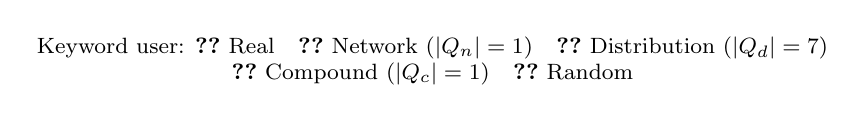
\begin{tikzpicture}
	\node [align=center, draw=none,font=\footnotesize, fill=none,anchor=north west] at (0,0) {Keyword user: \ref{plot:purple} Real\quad\ref{plot:dashdot} Network ($|Q_n|=1$)\quad\ref{plot:dashed} Distribution ($|Q_d|=7$) \\ \ref{plot:solid} Compound ($|Q_c|=1$)\quad\ref{plot:dotted} Random};
	\end{tikzpicture}
	
	
	\caption[Influence of similarity browsing on a ranking]{Influence of similarity browsing on a ranking. The horizontal axis shows position $t$ and the vertical axis shows probability $p(r\leq t)$ how likely random image will be in the first $t$ images given a query constructed by a given user and a number of re-rankings by the \textit{similarity} user with $D$ being the $50$ highest ranked images from the previous iteration or keyword initialization. Based on 1000 queries of the \textit{network}, the \textit{distribution} and the \textit{random} user, $1000+1000$ queries of the \textit{compound} user and 250~queries~of~the~\textit{real}~user.}
	\label{fig:simulation_rerank}
\end{figure}
\subsection{Similarity Re-Ranking}
Many interactive video retrieval tools enable a user to query a database in many modalities. The most relevant shots (images) $D$ are then displayed to the user. If searched image $\bm{x}$ is not present in the set $D$, usually the user can sequentially browse the results. However, as datasets get bigger this approach quickly becomes unfeasible. Retrieval systems, therefore, provide an option of similarity browsing based on handcrafted features or more recently deep neural network features~\cite{lokovc2018revisiting,barthel2018fusing} speeding up the search if visually and/or semantically similar image is present in the set $D$. Therefore we evaluate our model together with similarity browsing based on our networks deep features to better estimate the model's performance in the known-item search task. We take the definition of similarity user from \cite{kovalvcik2017comparison}:
\begin{description}[labelwidth=1em, leftmargin=!]
	\item Ideal \textbf{Similarity User.} Given a target image $\bm{x}$ and a set of the most relevant images $D$, the most similar image to $\bm{x}$ from $D$ is selected.
\end{description}
We define similarity of two images as the cosine of the angle between their activation values in the last average pooling layer of GoogLeNet denoted as $f'(\cdot;\bm{\theta})$:
\begin{equation}
similarity(\bm{a},\bm{b}) = \frac{\langle f'(\bm{a};\bm{\theta}),f'(\bm{b};\bm{\theta})\rangle}{\|f'(\bm{a};\bm{\theta})\|\|f'(\bm{b};\bm{\theta})\|}
\end{equation}
where $\bm{a}$ and $\bm{b}$ are two images, $\langle\cdot,\cdot\rangle$ is dot product and $\|\cdot\|$ is $L_2$ norm.

In the simulations the keyword users are used to assign each image in a collection initial rank, and $|D|$ top ranking images are passed to the similarity user. Even though, as reported by \cite{kovalvcik2017comparison}, humans usually do not select the most similar image based on our $similarity$ measure we can use this optimistic approximation to show theoretical limits of our model and to compare how well keyword initialization helps with the \textit{page zero problem} of similarity browsing.
Results in Figure \ref{fig:simulation_rerank} shows that one re-ranking significantly improves the chance of success whereas the added value of every other re-ranking lowers probably because we converge to some cluster in high dimensional feature space. We can also see that even given the \textit{network} keyword user and the ideal \textit{similarity} user 20\% of images we not found, therefore, proving interactive search using other approaches such as color or edge sketches as a necessity. With respect to the results of simulations with random query initialization, we argue that such small gap between the \textit{random} and the \textit{distribution} user after three re-rankings is due to target dataset's uniformity where keyword initialization cannot help much. This also supports conclusion of~\cite{kovalvcik2017comparison} that some images are unreachable by similarity re-ranking. Searching for dataset's distinct objects using only similarity browsing is on the other hand, based on our experience with the dataset, almost impossible.



\section{VBS Competition}

Since 2012, The Video Browser Showdown competition~\cite{cobarzan2017interactive,Lokoc-influential-trends}, organized at the \textit{International Conference on MultiMedia Modeling}, serves as a stage where researches evaluate their interactive video retrieval tools. SIRET group of Charles University debuted at the competition in 2014~\cite{Lokoc-VBS2014}, winning it in years 2014, 2015 and newly with our keyword-based retrieval model in 2018. Note that an older set of 1390 labels was used there. The set missed multiple key concepts and also contained many duplicate or very similar concepts thus we introduced the label clustering described in Chapter~\ref{sec:dataset_selection}. However, the rest stayed unchanged hence we can in this section introduce the competition and discuss our tool's results.

VBS competition focuses on known-item search (KIS) and ad-hoc video search (AVS) tasks in a highly interactive
way with a human in the loop rather than using only automated retrieval systems. Such a task can highly differ from just automated systems and maybe surprisingly some tools~\cite{Storyboard-Based_Interface,duane2018virtual} with little to no automated retrieval models can hold up to tools designed on deep learning models. In 2018, VBS comprised of three types of tasks on TRECVid's IACC.3 600 hour dataset~\cite{awad2016trecvid}: \textit{(1)} Visual known-item search (KIS) task with users searching short selected clip played in loop but with clip getting continually more and more blurred to prevent teams to focus on one image of the clip only. Also recording the played clip is forbidden since such a task is addressed in other computer vision benchmarks. \textit{(2)} Textual known-item search (KIS) task with users searching for short clip only described by text. Due to its inherent difficulty, more information appears over time. \textit{(3)} Ad-hoc search (AVS) task where users are given short text description and goals is to find as many scenes as possible corresponding to the description.

\subsection{Scoring}
For the visual and the textual KIS tasks the following formula was used at VBS 2018:
\begin{equation}
\max\left(0,\ 50 + 50\cdot\frac{t_L-t}{t_L} - 10\cdot\abs{WS}\right)
\end{equation}
where $t_L$ is the duration of the task (5 minutes for visual and 7 minutes for textual~KIS), $t$ is a time of submission and $\abs{WS}$ is a number of wrong submissions before the correct one. If there is not any correct submission sent in time, no points are awarded. For AVS task time-independent function was used:
\begin{equation}
\frac{|C|}{|C|+|I|/2}\cdot\frac{|q(C)|}{|q(P)|}
\end{equation}
where $|C|$ is a number of correct and $|I|$ a number of incorrect team's submissions and $P$ is set of all correct submissions by all teams representing an artificial recall~of~100\%. Function $q(\cdot)$ clusters shots of one scene into one frame encouraging teams to find different videos (or segments) rather than to send all frames of one scene (see~\cite{Lokoc-influential-trends} for a detailed explanation).

During the competition, there were five runs each with four tasks -- visual KIS, textual KIS and AVS rounds with tools being operated by experts (usually the creators of the tools) and another visual KIS and AVS rounds with tools operated by novice users selected from conference visitors. The overall score was determined by averaging all five rounds with a winner of each round getting 100 points and others proportionally to the winner.

\begin{table}
	
	\centering
	\sisetup{detect-weight=true,detect-inline-weight=math}
	\begin{tabular}{l@{\hspace{0.5cm}}S[table-format=3.0]S[table-format=3.0]S[table-format=3.0]S[table-format=3.0]S[table-format=3.0]S[table-format=3.0]}
		\toprule
		\multirow{2}{*}{\textbf{Team}} & \multicolumn{1}{c}{Visual} & \multicolumn{1}{c}{Textual} & \multicolumn{1}{c}{\multirow{2}{*}{AVS}} & \multicolumn{1}{c}{Visual KIS} & \multicolumn{1}{c}{AVS} & \multicolumn{1}{c}{\multirow{2}{*}{\textbf{Overall}}} \\
		& \multicolumn{1}{c}{KIS} & \multicolumn{1}{c}{KIS} & & \multicolumn{1}{c}{Novice} & \multicolumn{1}{c}{Novice} & \\
		\midrule
		SIRET (our)~\cite{lokovc2018revisiting}& 95\por{2}&\bftabnum 100\por{1}&    71\por{4}&           67\por{4}&    83\por{2}& \bftabnum 83\\
		ITEC1~\cite{ITEC1}      & 64\por{6}&           37\por{5}&    60\por{7}&\bftabnum 100\por{1}&    64\por{4}& 65\\
		ITEC2~\cite{ITEC2}      & 29\por{8}&           47\por{3}&    81\por{2}&           85\por{3}&    75\por{3}& 63\\
		HTW~\cite{barthel2018fusing}        & 91\por{3}&           41\por{4}&    61\por{6}&           50\por{5}&    61\por{5}& 61\\
		NECTEC~\cite{NECTEC}     & 68\por{5}&            0&\bftabnum 100\por{1}&            0&\bftabnum 100\por{1}& 54\\
		VIREO~\cite{VIREO}      &\bftabnum 100\por{1}&  0&           50\por{8}&           86\por{2}&    30\por{8}& 53\\
		VITRIVR~\cite{VITRIVR}    & 79\por{4}&           55\por{2}&    64\por{5}&            0&           35\por{7}& 47\\
		VERGE~\cite{VERGE}      & 62\por{7}&            0&           72\por{3}&            0&           46\por{6}& 36\\
		VNU~\cite{VNU}        & 21\por{9}&            0&           41\por{9}&           48\por{6}&    14\por{9}& 25\\
		\bottomrule
		\multicolumn{7}{l}{\footnotesize ($\cdot$) Standing in individual round.}
	\end{tabular}
	
	\caption[VBS 2018 results]{VBS 2018 results.}
	\label{fig:vbs_results}
\end{table}

\begin{table}[b!]
	\centering
	\sisetup{detect-weight=true,detect-inline-weight=math}
	\begin{tabular}{cccc|cccc|cccc|cccc|cccc}
		\toprule
		$\substack{V \\ E}$ & $\substack{V \\ E}$ & $\substack{V \\ E}$ & $\substack{V \\ E}$ & $\substack{T \\ E}$ & $\substack{T \\ E}$ & $\substack{T \\ E}$ & $\substack{T \\ E}$ & $\substack{A \\ E}$ & $\substack{A \\ E}$ & $\substack{A \\ E}$ & $\substack{A \\ E}$ & $\substack{V \\ N}$ & $\substack{V \\ N}$ & $\substack{V \\ N}$ & $\substack{V \\ N}$ & $\substack{A \\ N}$ & $\substack{A \\ N}$ & $\substack{A \\ N}$ & $\substack{A \\ N}$ \\
		\midrule
		2 & 4 & 8 & 7 & \textcolor{red}{0} & 3 & \textcolor{red}{0} & 3 & 9 & 9 & 9 & 9 & \textcolor{red}{1} & 3 & 4 & \textcolor{red}{3} & 9 & 9 & 9 & 8 \\
		\bottomrule
	\end{tabular}
	
	\caption[Number of successful teams per task at VBS 2018]{A number of successful teams per video KIS (V), textual KIS (T) and AVS~(A) task with the tool being operated by experts (E) or novices (N). Red tasks were not solved by our tool.}
	\label{fig:vbs_tasks}
\end{table}

\subsection{Results}
The results of VBS 2018 are presented in Table \ref{fig:vbs_results} where it can be seen we won by significant margin scoring 27 percent more points than the second team. However, in Table \ref{fig:vbs_tasks_timeline}, we can see there are still areas for improvement especially in the textual KIS tasks where two of the four tasks were not solved by any team. But we can proudly report that SIRET was the only team to successfully solve both solved textual KIS tasks and all expert visual KIS task even though we finished the round second after a team with only three solved tasks because of the wrong submission penalty in the first task. Interestingly even though strong in the expert visual run, in the novice run we were not able to solve two out of four tasks. This trend of lower performance in novice run can be however observed with all teams except ITEC1 and ITEC2 with the former being the only team solving three out of four tasks.


Since VBS 2018 mandatory logging of user actions was established such that with each frame sent to the server basic set of actions that lead to the result was submitted. Even though a complete analysis will be published in a separate journal, we can at least show and analyze logs from our tool presented in Figure~\ref{fig:vbs_tasks_timeline}. Looking at the visual KIS expert tasks, we can see that both keyword and color sketch can be the equally good initialization of a display from which we can semantically browse the collection. On the other hand in the textual KIS tasks, keyword plays the utmost role in success with all teams starting with keyword queries except ITEC2 which utilized their advanced color sketch interface but in the end falling back on keyword search anyway. When comparing expert and novice users, we can see the expert's more systematic approach utilizing fewer models at once. At least in the second and fourth expert visual task, we can with high probability say a user has been systematically using the color sketch as a filter wheres novices with their rapid model changes could hardly do some systematic filtering. The AVS tasks show the dominance of keyword search with the most of the tasks being solved without using any other model. Visual representation of AVS logs can be seen in the Attachment \ref{att:vbs_tasks_timeline_avs}.

\begin{figure}
	\centering
	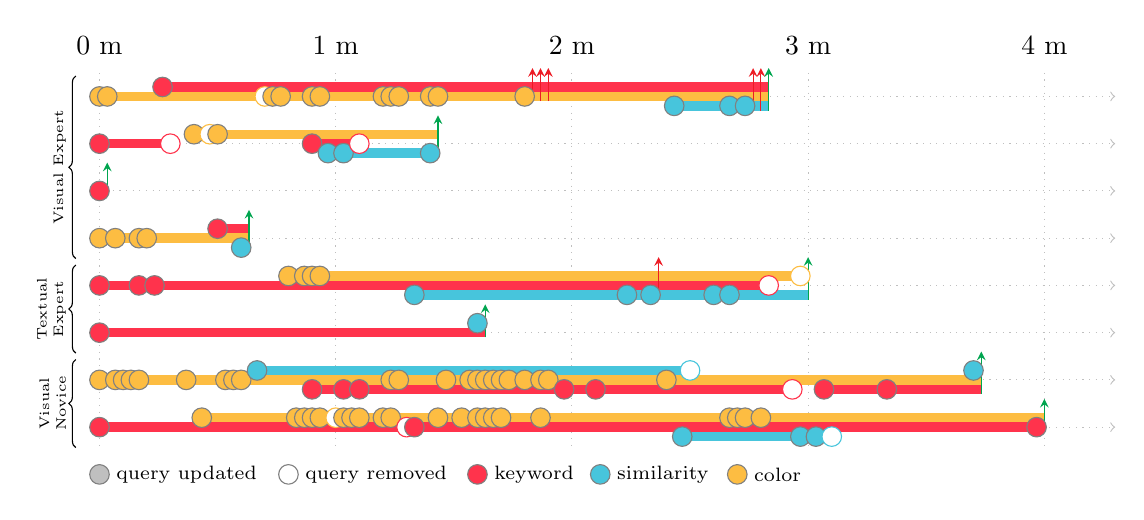
\begin{tikzpicture}[scale=2,x=1.5cm]
\usetikzlibrary{shapes}
\definecolor{YellowGreen}{RGB}{255,51,76}
\definecolor{SkyBlue}{RGB}{71,197,220}
\definecolor{Green}{RGB}{0,165,79}
\definecolor{Red}{RGB}{237,27,36}
\definecolor{Dandelion}{RGB}{253,189,66}
% draw horizontal line   
\draw[->,dotted,lightgray] (0,-0.150) -- (4.3,-0.150); 

\draw[->,dotted,lightgray] (0,-0.450) -- (4.3,-0.450); 

\draw[->,dotted,lightgray] (0,-0.750) -- (4.3,-0.750); 

\draw[->,dotted,lightgray] (0,-1.050) -- (4.3,-1.050); 

\draw[->,dotted,lightgray] (0,-1.350) -- (4.3,-1.350); 

\draw[->,dotted,lightgray] (0,-1.650) -- (4.3,-1.650); 

\draw[->,dotted,lightgray] (0,-1.950) -- (4.3,-1.950); 

\draw[->,dotted,lightgray] (0,-2.250) -- (4.3,-2.250);

% draw vertical lines
\foreach \x in {0,1,2,3,4}
\draw[dotted,lightgray] (\x,0) -- (\x,-2.40);

% draw nodes
\draw (0,0) node[above=3pt] {0 m};
\draw (1,0) node[above=3pt] {1 m};
\draw (2,0) node[above=3pt] {2 m};
\draw (3,0) node[above=3pt] {3 m};
\draw (4,0) node[above=3pt] {4 m};

\draw[decorate,decoration={brace}] (-0.1,-1.18) -- (-0.1,-0.02) node[midway, anchor=center, sloped, above=0.1, font=\tiny, align=center] {Visual Expert};
\draw[decorate,decoration={brace}] (-0.1,-1.78) -- (-0.1,-1.22) node[midway, anchor=center, sloped, above=0.1, font=\tiny, align=center] {Textual \\ Expert};
\draw[decorate,decoration={brace}] (-0.1,-2.38) -- (-0.1,-1.82) node[midway, anchor=center, sloped, above=0.1, font=\tiny, align=center] {Visual \\ Novice};

\node[draw=gray, circle, fill=lightgray, inner sep=2.5pt, align=center]at (0,-2.55) {};
\node[anchor=west, font=\scriptsize]at (0.03,-2.55) {query updated};
\node[draw=gray, circle, fill=white, inner sep=2.5pt, align=center]at (0.8,-2.55) {};
\node[anchor=west, font=\scriptsize]at (0.83,-2.55) {query removed};

\node[draw=gray, circle, fill=YellowGreen, inner sep=2.5pt, align=center]at (1.6,-2.55) {};
\node[anchor=west, font=\scriptsize]at (1.63,-2.55) {keyword};
\node[draw=gray, circle, fill=SkyBlue, inner sep=2.5pt, align=center]at (2.12,-2.55) {};
\node[anchor=west, font=\scriptsize]at (2.15,-2.55) {similarity};
\node[draw=gray, circle, fill=Dandelion, inner sep=2.5pt, align=center]at (2.7,-2.55) {};
\node[anchor=west, font=\scriptsize]at (2.73,-2.55) {color};

\draw[line width=0.12cm, Dandelion](0.000,-0.150 -0) -- (0.700,-0.150 -0);
\draw[line width=0.12cm, YellowGreen](0.267,-0.150 +0.06) -- (2.833,-0.150 +0.06);
\draw[line width=0.12cm, Dandelion](0.733,-0.150 -0) -- (2.833,-0.150 -0);
\draw[line width=0.12cm, SkyBlue](2.433,-0.150 -0.06) -- (2.833,-0.150 -0.06);
\draw[-stealth,Red] (1.833,-0.150 -0.03) -- (1.833,-0.150 + 0.18);
\draw[-stealth,Red] (1.867,-0.150 -0.03) -- (1.867,-0.150 + 0.18);
\draw[-stealth,Red] (1.900,-0.150 -0.03) -- (1.900,-0.150 + 0.18);
\draw[-stealth,Red] (2.767,-0.150 -0.09) -- (2.767,-0.150 + 0.18);
\draw[-stealth,Red] (2.800,-0.150 -0.09) -- (2.800,-0.150 + 0.18);
\draw[-stealth,Green] (2.833,-0.150 -0.09) -- (2.833,-0.150 + 0.18);
\node[draw=gray, circle, fill=Dandelion, inner sep=2.5pt, align=center]at (0.000,-0.150 -0) {};
\node[draw=gray, circle, fill=Dandelion, inner sep=2.5pt, align=center]at (0.033,-0.150 -0) {};
\node[draw=gray, circle, fill=YellowGreen, inner sep=2.5pt, align=center]at (0.267,-0.150 +0.06) {};
\node[draw=Dandelion, circle, fill=white, inner sep=2.5pt, align=center]at (0.700,-0.150 -0) {};
\node[draw=gray, circle, fill=Dandelion, inner sep=2.5pt, align=center]at (0.733,-0.150 -0) {};
\node[draw=gray, circle, fill=Dandelion, inner sep=2.5pt, align=center]at (0.767,-0.150 -0) {};
\node[draw=gray, circle, fill=Dandelion, inner sep=2.5pt, align=center]at (0.900,-0.150 -0) {};
\node[draw=gray, circle, fill=Dandelion, inner sep=2.5pt, align=center]at (0.933,-0.150 -0) {};
\node[draw=gray, circle, fill=Dandelion, inner sep=2.5pt, align=center]at (1.200,-0.150 -0) {};
\node[draw=gray, circle, fill=Dandelion, inner sep=2.5pt, align=center]at (1.233,-0.150 -0) {};
\node[draw=gray, circle, fill=Dandelion, inner sep=2.5pt, align=center]at (1.267,-0.150 -0) {};
\node[draw=gray, circle, fill=Dandelion, inner sep=2.5pt, align=center]at (1.400,-0.150 -0) {};
\node[draw=gray, circle, fill=Dandelion, inner sep=2.5pt, align=center]at (1.433,-0.150 -0) {};
\node[draw=gray, circle, fill=Dandelion, inner sep=2.5pt, align=center]at (1.800,-0.150 -0) {};
\node[draw=gray, circle, fill=SkyBlue, inner sep=2.5pt, align=center]at (2.433,-0.150 -0.06) {};
\node[draw=gray, circle, fill=SkyBlue, inner sep=2.5pt, align=center]at (2.667,-0.150 -0.06) {};
\node[draw=gray, circle, fill=SkyBlue, inner sep=2.5pt, align=center]at (2.733,-0.150 -0.06) {};


\draw[line width=0.12cm, YellowGreen](0.000,-0.450 -0) -- (0.300,-0.450 -0);
\draw[line width=0.12cm, Dandelion](0.400,-0.450 +0.06) -- (0.467,-0.450 +0.06);
\draw[line width=0.12cm, YellowGreen](0.900,-0.450 -0) -- (1.100,-0.450 -0);
\draw[line width=0.12cm, Dandelion](0.500,-0.450 +0.06) -- (1.433,-0.450 +0.06);
\draw[line width=0.12cm, SkyBlue](0.967,-0.450 -0.06) -- (1.433,-0.450 -0.06);
\draw[-stealth,Green] (1.433,-0.450 -0.09) -- (1.433,-0.450 + 0.18);
\node[draw=gray, circle, fill=YellowGreen, inner sep=2.5pt, align=center]at (0.000,-0.450 -0) {};
\node[draw=YellowGreen, circle, fill=white, inner sep=2.5pt, align=center]at (0.300,-0.450 -0) {};
\node[draw=gray, circle, fill=Dandelion, inner sep=2.5pt, align=center]at (0.400,-0.450 +0.06) {};
\node[draw=Dandelion, circle, fill=white, inner sep=2.5pt, align=center]at (0.467,-0.450 +0.06) {};
\node[draw=gray, circle, fill=Dandelion, inner sep=2.5pt, align=center]at (0.500,-0.450 +0.06) {};
\node[draw=gray, circle, fill=YellowGreen, inner sep=2.5pt, align=center]at (0.900,-0.450 -0) {};
\node[draw=gray, circle, fill=SkyBlue, inner sep=2.5pt, align=center]at (0.967,-0.450 -0.06) {};
\node[draw=gray, circle, fill=SkyBlue, inner sep=2.5pt, align=center]at (1.033,-0.450 -0.06) {};
\node[draw=YellowGreen, circle, fill=white, inner sep=2.5pt, align=center]at (1.100,-0.450 -0) {};
\node[draw=gray, circle, fill=SkyBlue, inner sep=2.5pt, align=center]at (1.400,-0.450 -0.06) {};


\draw[line width=0.12cm, YellowGreen](0.000,-0.750 -0) -- (0.033,-0.750 -0);
\draw[-stealth,Green] (0.033,-0.750) -- (0.033,-0.750 + 0.18);
\node[draw=gray, circle, fill=YellowGreen, inner sep=2.5pt, align=center]at (0.000,-0.750 -0) {};


\draw[line width=0.12cm, YellowGreen](0.500,-1.050 +0.06) -- (0.633,-1.050 +0.06);
\draw[line width=0.12cm, Dandelion](0.000,-1.050 -0) -- (0.633,-1.050 -0);
\draw[line width=0.12cm, SkyBlue](0.600,-1.050 -0.06) -- (0.633,-1.050 -0.06);
\draw[-stealth,Green] (0.633,-1.050 -0.09) -- (0.633,-1.050 + 0.18);
\node[draw=gray, circle, fill=Dandelion, inner sep=2.5pt, align=center]at (0.000,-1.050 -0) {};
\node[draw=gray, circle, fill=Dandelion, inner sep=2.5pt, align=center]at (0.067,-1.050 -0) {};
\node[draw=gray, circle, fill=Dandelion, inner sep=2.5pt, align=center]at (0.167,-1.050 -0) {};
\node[draw=gray, circle, fill=Dandelion, inner sep=2.5pt, align=center]at (0.200,-1.050 -0) {};
\node[draw=gray, circle, fill=YellowGreen, inner sep=2.5pt, align=center]at (0.500,-1.050 +0.06) {};
\node[draw=gray, circle, fill=SkyBlue, inner sep=2.5pt, align=center]at (0.600,-1.050 -0.06) {};


\draw[line width=0.12cm, YellowGreen](0.000,-1.350 -0) -- (2.833,-1.350 -0);
\draw[line width=0.12cm, Dandelion](0.800,-1.350 +0.06) -- (2.967,-1.350 +0.06);
\draw[line width=0.12cm, SkyBlue](1.333,-1.350 -0.06) -- (3.000,-1.350 -0.06);
\draw[-stealth,Red] (2.367,-1.350 -0.09) -- (2.367,-1.350 + 0.18);
\draw[-stealth,Green] (3.000,-1.350 -0.09) -- (3.000,-1.350 + 0.18);
\node[draw=gray, circle, fill=YellowGreen, inner sep=2.5pt, align=center]at (0.000,-1.350 -0) {};
\node[draw=gray, circle, fill=YellowGreen, inner sep=2.5pt, align=center]at (0.167,-1.350 -0) {};
\node[draw=gray, circle, fill=YellowGreen, inner sep=2.5pt, align=center]at (0.233,-1.350 -0) {};
\node[draw=gray, circle, fill=Dandelion, inner sep=2.5pt, align=center]at (0.800,-1.350 +0.06) {};
\node[draw=gray, circle, fill=Dandelion, inner sep=2.5pt, align=center]at (0.867,-1.350 +0.06) {};
\node[draw=gray, circle, fill=Dandelion, inner sep=2.5pt, align=center]at (0.900,-1.350 +0.06) {};
\node[draw=gray, circle, fill=Dandelion, inner sep=2.5pt, align=center]at (0.933,-1.350 +0.06) {};
\node[draw=gray, circle, fill=SkyBlue, inner sep=2.5pt, align=center]at (1.333,-1.350 -0.06) {};
\node[draw=gray, circle, fill=SkyBlue, inner sep=2.5pt, align=center]at (2.233,-1.350 -0.06) {};
\node[draw=gray, circle, fill=SkyBlue, inner sep=2.5pt, align=center]at (2.333,-1.350 -0.06) {};
\node[draw=gray, circle, fill=SkyBlue, inner sep=2.5pt, align=center]at (2.600,-1.350 -0.06) {};
\node[draw=gray, circle, fill=SkyBlue, inner sep=2.5pt, align=center]at (2.667,-1.350 -0.06) {};
\node[draw=YellowGreen, circle, fill=white, inner sep=2.5pt, align=center]at (2.833,-1.350 -0) {};
\node[draw=Dandelion, circle, fill=white, inner sep=2.5pt, align=center]at (2.967,-1.350 +0.06) {};


\draw[line width=0.12cm, SkyBlue](1.600,-1.650 +0.06) -- (1.633,-1.650 +0.06);
\draw[line width=0.12cm, YellowGreen](0.000,-1.650 -0) -- (1.633,-1.650 -0);
\draw[-stealth,Green] (1.633,-1.650-0.03) -- (1.633,-1.650 + 0.18);
\node[draw=gray, circle, fill=YellowGreen, inner sep=2.5pt, align=center]at (0.000,-1.650 -0) {};
\node[draw=gray, circle, fill=SkyBlue, inner sep=2.5pt, align=center]at (1.600,-1.650 +0.06) {};


\draw[line width=0.12cm, SkyBlue](0.667,-1.950 +0.06) -- (2.500,-1.950 +0.06);
\draw[line width=0.12cm, YellowGreen](0.900,-1.950 -0.06) -- (2.933,-1.950 -0.06);
\draw[line width=0.12cm, SkyBlue](3.700,-1.950 +0.06) -- (3.733,-1.950 +0.06);
\draw[line width=0.12cm, Dandelion](0.000,-1.950 -0) -- (3.733,-1.950 -0);
\draw[line width=0.12cm, YellowGreen](3.067,-1.950 -0.06) -- (3.733,-1.950 -0.06);
\draw[-stealth,Green] (3.733,-1.950 -0.09) -- (3.733,-1.950 + 0.18);
\node[draw=gray, circle, fill=Dandelion, inner sep=2.5pt, align=center]at (0.000,-1.950 -0) {};
\node[draw=gray, circle, fill=Dandelion, inner sep=2.5pt, align=center]at (0.067,-1.950 -0) {};
\node[draw=gray, circle, fill=Dandelion, inner sep=2.5pt, align=center]at (0.100,-1.950 -0) {};
\node[draw=gray, circle, fill=Dandelion, inner sep=2.5pt, align=center]at (0.133,-1.950 -0) {};
\node[draw=gray, circle, fill=Dandelion, inner sep=2.5pt, align=center]at (0.167,-1.950 -0) {};
\node[draw=gray, circle, fill=Dandelion, inner sep=2.5pt, align=center]at (0.367,-1.950 -0) {};
\node[draw=gray, circle, fill=Dandelion, inner sep=2.5pt, align=center]at (0.533,-1.950 -0) {};
\node[draw=gray, circle, fill=Dandelion, inner sep=2.5pt, align=center]at (0.567,-1.950 -0) {};
\node[draw=gray, circle, fill=Dandelion, inner sep=2.5pt, align=center]at (0.600,-1.950 -0) {};
\node[draw=gray, circle, fill=SkyBlue, inner sep=2.5pt, align=center]at (0.667,-1.950 +0.06) {};
\node[draw=gray, circle, fill=YellowGreen, inner sep=2.5pt, align=center]at (0.900,-1.950 -0.06) {};
\node[draw=gray, circle, fill=YellowGreen, inner sep=2.5pt, align=center]at (1.033,-1.950 -0.06) {};
\node[draw=gray, circle, fill=YellowGreen, inner sep=2.5pt, align=center]at (1.100,-1.950 -0.06) {};
\node[draw=gray, circle, fill=Dandelion, inner sep=2.5pt, align=center]at (1.233,-1.950 -0) {};
\node[draw=gray, circle, fill=Dandelion, inner sep=2.5pt, align=center]at (1.267,-1.950 -0) {};
\node[draw=gray, circle, fill=Dandelion, inner sep=2.5pt, align=center]at (1.467,-1.950 -0) {};
\node[draw=gray, circle, fill=Dandelion, inner sep=2.5pt, align=center]at (1.567,-1.950 -0) {};
\node[draw=gray, circle, fill=Dandelion, inner sep=2.5pt, align=center]at (1.600,-1.950 -0) {};
\node[draw=gray, circle, fill=Dandelion, inner sep=2.5pt, align=center]at (1.633,-1.950 -0) {};
\node[draw=gray, circle, fill=Dandelion, inner sep=2.5pt, align=center]at (1.667,-1.950 -0) {};
\node[draw=gray, circle, fill=Dandelion, inner sep=2.5pt, align=center]at (1.700,-1.950 -0) {};
\node[draw=gray, circle, fill=Dandelion, inner sep=2.5pt, align=center]at (1.733,-1.950 -0) {};
\node[draw=gray, circle, fill=Dandelion, inner sep=2.5pt, align=center]at (1.800,-1.950 -0) {};
\node[draw=gray, circle, fill=Dandelion, inner sep=2.5pt, align=center]at (1.867,-1.950 -0) {};
\node[draw=gray, circle, fill=Dandelion, inner sep=2.5pt, align=center]at (1.900,-1.950 -0) {};
\node[draw=gray, circle, fill=YellowGreen, inner sep=2.5pt, align=center]at (1.967,-1.950 -0.06) {};
\node[draw=gray, circle, fill=YellowGreen, inner sep=2.5pt, align=center]at (2.100,-1.950 -0.06) {};
\node[draw=gray, circle, fill=Dandelion, inner sep=2.5pt, align=center]at (2.400,-1.950 -0) {};
\node[draw=SkyBlue, circle, fill=white, inner sep=2.5pt, align=center]at (2.500,-1.950 +0.06) {};
\node[draw=YellowGreen, circle, fill=white, inner sep=2.5pt, align=center]at (2.933,-1.950 -0.06) {};
\node[draw=gray, circle, fill=YellowGreen, inner sep=2.5pt, align=center]at (3.067,-1.950 -0.06) {};
\node[draw=gray, circle, fill=YellowGreen, inner sep=2.5pt, align=center]at (3.333,-1.950 -0.06) {};
\node[draw=gray, circle, fill=SkyBlue, inner sep=2.5pt, align=center]at (3.700,-1.950 +0.06) {};


\draw[line width=0.12cm, Dandelion](0.433,-2.250 +0.06) -- (1.000,-2.250 +0.06);
\draw[line width=0.12cm, YellowGreen](0.000,-2.250 -0) -- (1.300,-2.250 -0);
\draw[line width=0.12cm, SkyBlue](2.467,-2.250 -0.06) -- (3.100,-2.250 -0.06);
\draw[line width=0.12cm, Dandelion](1.033,-2.250 +0.06) -- (4.000,-2.250 +0.06);
\draw[line width=0.12cm, YellowGreen](1.333,-2.250 -0) -- (4.000,-2.250 -0);
\draw[-stealth,Green] (4.000,-2.250) -- (4.000,-2.250 + 0.18);
\node[draw=gray, circle, fill=YellowGreen, inner sep=2.5pt, align=center]at (0.000,-2.250 -0) {};
\node[draw=gray, circle, fill=Dandelion, inner sep=2.5pt, align=center]at (0.433,-2.250 +0.06) {};
\node[draw=gray, circle, fill=Dandelion, inner sep=2.5pt, align=center]at (0.833,-2.250 +0.06) {};
\node[draw=gray, circle, fill=Dandelion, inner sep=2.5pt, align=center]at (0.867,-2.250 +0.06) {};
\node[draw=gray, circle, fill=Dandelion, inner sep=2.5pt, align=center]at (0.900,-2.250 +0.06) {};
\node[draw=gray, circle, fill=Dandelion, inner sep=2.5pt, align=center]at (0.933,-2.250 +0.06) {};
\node[draw=Dandelion, circle, fill=white, inner sep=2.5pt, align=center]at (1.000,-2.250 +0.06) {};
\node[draw=gray, circle, fill=Dandelion, inner sep=2.5pt, align=center]at (1.033,-2.250 +0.06) {};
\node[draw=gray, circle, fill=Dandelion, inner sep=2.5pt, align=center]at (1.067,-2.250 +0.06) {};
\node[draw=gray, circle, fill=Dandelion, inner sep=2.5pt, align=center]at (1.100,-2.250 +0.06) {};
\node[draw=gray, circle, fill=Dandelion, inner sep=2.5pt, align=center]at (1.200,-2.250 +0.06) {};
\node[draw=gray, circle, fill=Dandelion, inner sep=2.5pt, align=center]at (1.233,-2.250 +0.06) {};
\node[draw=YellowGreen, circle, fill=white, inner sep=2.5pt, align=center]at (1.300,-2.250 -0) {};
\node[draw=gray, circle, fill=YellowGreen, inner sep=2.5pt, align=center]at (1.333,-2.250 -0) {};
\node[draw=gray, circle, fill=Dandelion, inner sep=2.5pt, align=center]at (1.433,-2.250 +0.06) {};
\node[draw=gray, circle, fill=Dandelion, inner sep=2.5pt, align=center]at (1.533,-2.250 +0.06) {};
\node[draw=gray, circle, fill=Dandelion, inner sep=2.5pt, align=center]at (1.600,-2.250 +0.06) {};
\node[draw=gray, circle, fill=Dandelion, inner sep=2.5pt, align=center]at (1.633,-2.250 +0.06) {};
\node[draw=gray, circle, fill=Dandelion, inner sep=2.5pt, align=center]at (1.667,-2.250 +0.06) {};
\node[draw=gray, circle, fill=Dandelion, inner sep=2.5pt, align=center]at (1.700,-2.250 +0.06) {};
\node[draw=gray, circle, fill=Dandelion, inner sep=2.5pt, align=center]at (1.867,-2.250 +0.06) {};
\node[draw=gray, circle, fill=SkyBlue, inner sep=2.5pt, align=center]at (2.467,-2.250 -0.06) {};
\node[draw=gray, circle, fill=Dandelion, inner sep=2.5pt, align=center]at (2.667,-2.250 +0.06) {};
\node[draw=gray, circle, fill=Dandelion, inner sep=2.5pt, align=center]at (2.700,-2.250 +0.06) {};
\node[draw=gray, circle, fill=Dandelion, inner sep=2.5pt, align=center]at (2.733,-2.250 +0.06) {};
\node[draw=gray, circle, fill=Dandelion, inner sep=2.5pt, align=center]at (2.800,-2.250 +0.06) {};
\node[draw=gray, circle, fill=SkyBlue, inner sep=2.5pt, align=center]at (2.967,-2.250 -0.06) {};
\node[draw=gray, circle, fill=SkyBlue, inner sep=2.5pt, align=center]at (3.033,-2.250 -0.06) {};
\node[draw=SkyBlue, circle, fill=white, inner sep=2.5pt, align=center]at (3.100,-2.250 -0.06) {};
\node[draw=gray, circle, fill=YellowGreen, inner sep=2.5pt, align=center]at (3.967,-2.250 -0) {};
\end{tikzpicture}

	
	\caption[Use of tool's retrieval models in KIS tasks]{Use of our tool's retrieval models in all solved visual and textual KIS task at VBS 2018. The horizontal axis represents time since the task's start, green and red arrows represent correct and incorrect submissions to the competition's server.}
	\label{fig:vbs_tasks_timeline}
\end{figure}
